\documentclass{scrreprt}
\usepackage{listings}
\usepackage{underscore}
\usepackage[bookmarks=true]{hyperref}
\usepackage[utf8]{inputenc}
\usepackage[french]{babel}
\usepackage[top=2cm, bottom=3.5cm, left=3cm, right=3cm]{geometry}
\usepackage{fontawesome}
\usepackage[utf8]{inputenc}
\usepackage{array}
%\usepackage[latin1]{inputenc}
%\usepackage[francais]{babel}
\usepackage{graphicx}
\usepackage{titlesec}
\usepackage{multirow}

\setcounter{secnumdepth}{4}
\setcounter{tocdepth}{4}

\hypersetup{
    bookmarks=false,    % show bookmarks bar?
    pdftitle={Rapport},    % title
    pdfauthor={CRAPANZANO/TARDIVON},   % author
    pdfsubject={TeX and LaTeX},                        % subject of the document
    pdfkeywords={TeX, LaTeX, graphics, images}, % list of keywords
    colorlinks=true,       % false: boxed links; true: colored links
    linkcolor=black,       % color of internal links
    citecolor=black,       % color of links to bibliography
    filecolor=black,        % color of file links
    urlcolor=blue,        % color of external links
    linktoc=section            % only page is linked
}%
\def\myversion{1.0}
\date{}
%\title

\usepackage{hyperref}
%\usepackage[T1]{fontenc}
\begin{document}
%   TEST POUR AFFICHER L'IMAGE TELECOM NANCY
%\includegraphics[height=50px, width=100px]{Telecomnancy.png}
%
\thispagestyle{empty}
\begin{flushright}
    \rule{15cm}{3pt}\vskip1,5cm
    \begin{bfseries}
        \Huge{Project Report: \\ English}\\
        \vspace{2cm}
        \vspace{2cm}
        \Huge{Story-Branch}\\

        \vspace{0.5cm}
        \LARGE{Version \myversion}\\
        \begin{flushleft}
            \vspace{8cm}
            Github repository : \href{https://github.com/quentin-tardivon/Story-Branch}{\faGithub}~\\
            \vspace{0.5cm}

            Claire CRAPANZANO\\
            Quentin TARDIVON\\
        \end{flushleft}
    \end{bfseries}
\end{flushright}

\tableofcontents

\setcounter{page}{0}

\chapter{- Introduction}

For our English Project, we did not wish to make a tool whose purpose would have been to improve our grammar, vocabulary or pronunciation, but rather an application which would enlarge our knowledge about England's history. We were also inspired by \textit{Reigns}, a game in which you are a monarch and you have to take decisions to rule your country and make everyone happy to stay on the throne.
With this in mind, we sought to conciliate both by choosing to apply a derivative of this game principle on an era pretty well unknown : the Hundred Years War - which has to added benefit of being part of France's history too. That is how we conceived \textit{Story Branch}, our application.

{\let\clearpage\relax \chapter{- User Manual}}

\section{Preliminary searches}

\subsection*{}To find an idea for this project, we brainstormed after having agreed not to make an application that would be too scholastic ; namely, applications basing themselves on the memorization of words or grammar point. We found the idea of a game about English history very fitting, as it would make people learn about its culture a bit, which we consider to be also important when learning a foreign language.

\subsection*{} We had \textit{Reigns} in mind when we began, but the system with several bars representing the clergy, people and military seemed too complicated to implement on such a short time, notwithstanding the fact that every event is accompanied by an illustration - \textit{Reigns} is, after all, a paying game made by a real company. So, we wanted to keep the idea of being a monarch making choices, but ruled out the "Yes/No" system of Reigns to end up with three choices for each event ; we made a script for that entirely from scratch, but we will get to that latter.

Our choice for the era was the Hundred Years War, because it is a subject we both studied very little in class, but that lasted a pretty long time and is relevant to both France and England. Moreover, we found many sources of information, which eased our research process.

We almost immediately settled on the name \textit{Story Branch} because of a few reasons ; firstly, it really represented the concept behind our application, as the story really branches, and secondly, it sounded easy to understand and to remember.

\subsection*{}The principle of \textit{Story Branch} is quite simple : you play as the Kings of England throughout the Hundred Years War (Richard II, Edward III, Henry IV, V or VI according to where you are in the story), and you have events, that happened in real life, which you need to handle ; to do that, you must choose between three pre-made choices. The goal is to stick as closely as possible to real life, and your score is based on that. However, it is not just about choosing between two bad choices and one good, because some choices make you go forward in the story by skipping some events, some make you make even more wrong choices, and some even trigger "Game Over" !

\section{The script}

\subsection*{} To make the core story of our game, we had no choice but to look up the history of the Kings of England. One by one, we tried to outline their life to keep what was important and relevant. We did that "by hand", as we did not find a summary as we wanted, but that allowed us to really learn about England's history and story-telling as a whole. Once we narrowed it to what we considered important and implementable in the game, we had to come up with two bad choices for each event, which proved sometimes quite a challenge. To keep things interesting, we made little jokes and made sure to almost always propose a more reasonable choice than what happened in real life.
\subsection*{} The script finally amounts to 310 lines, and we have a total of 25 events, which makes 75 choices - more or less the ones you can skip by taking the right option. We thought that it was a good number, because it makes the game not too short and not too long. Here are a few pictures of the architecture the story have by King - beware of spoilers!

\begin{figure}
	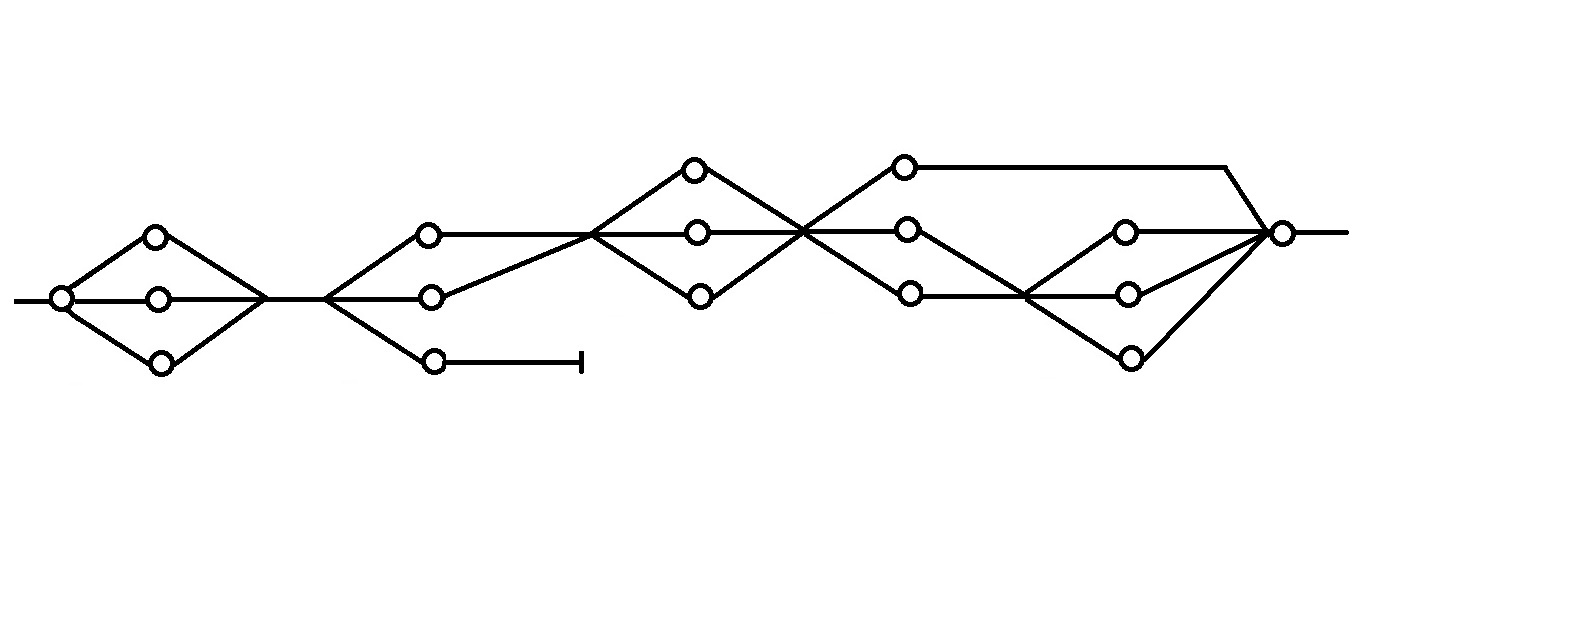
\includegraphics[scale=0.7]{Edward3.jpg}
	\begin{center}
		Decision tree for Edward III
	\end{center}
\end{figure}

\begin{figure}
	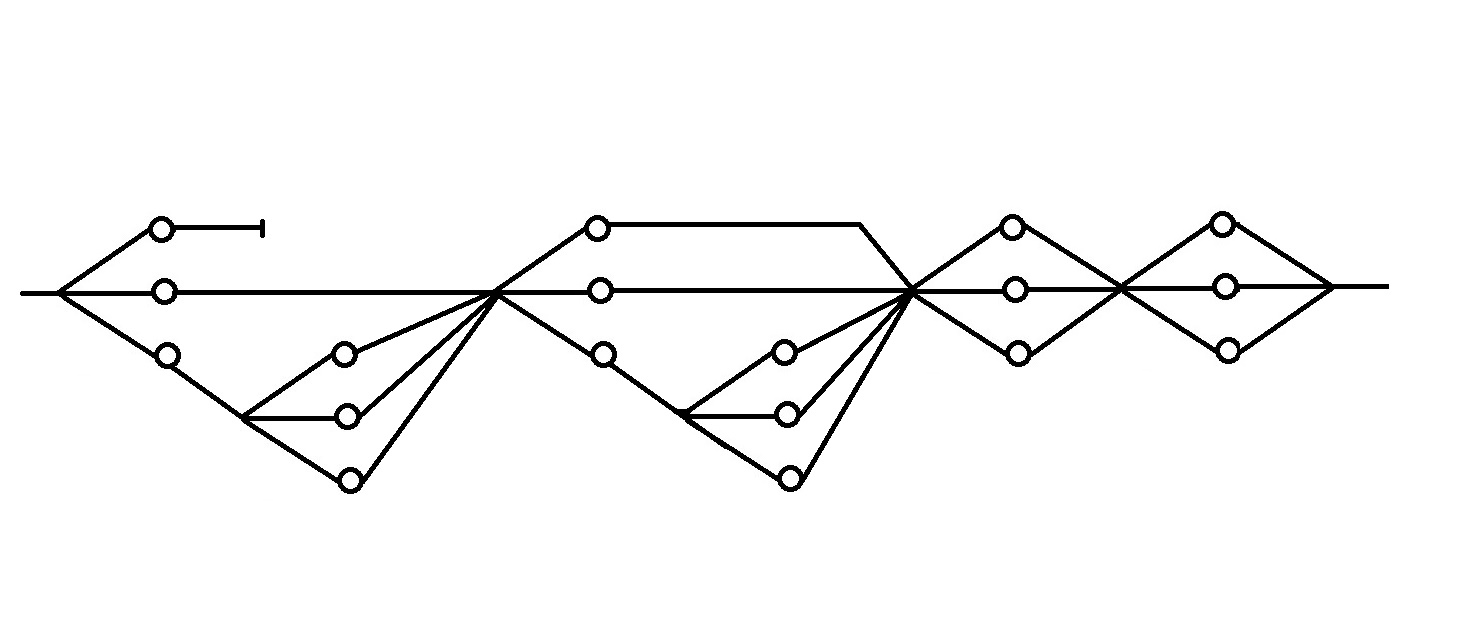
\includegraphics[scale=0.7]{Richard2.jpg}
	\begin{center}
		Decision tree for Richard II
	\end{center}
\end{figure}

\begin{figure}
	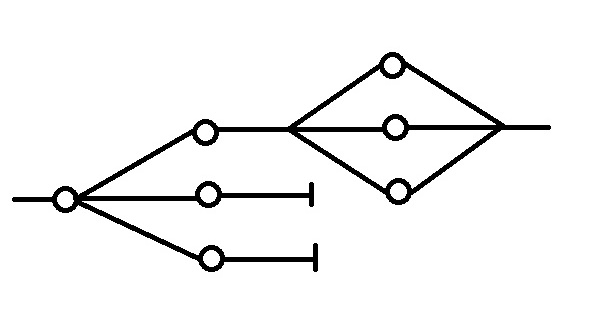
\includegraphics{Henry4Paint.jpg}
	\begin{center}
		Decision tree for Henry IV
	\end{center}
\end{figure}

\begin{figure}
	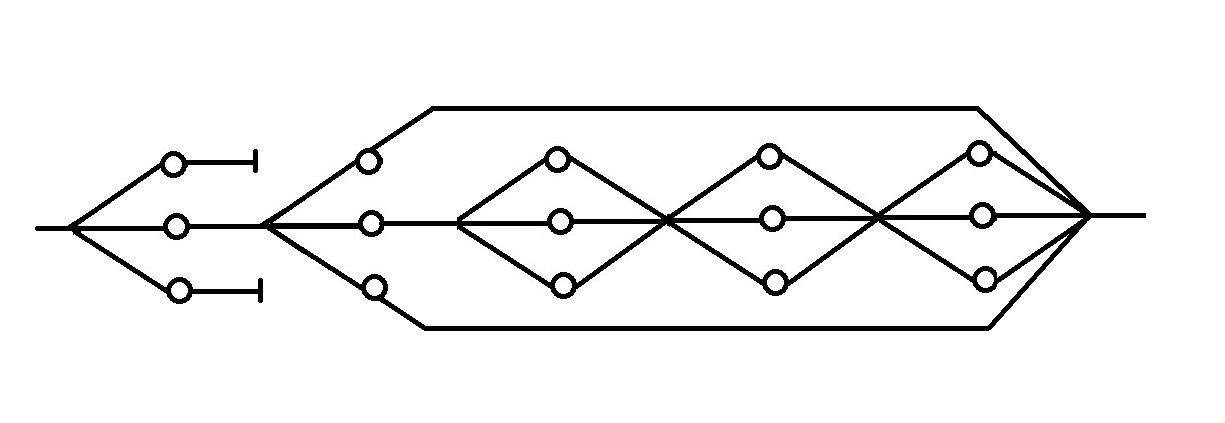
\includegraphics[scale=0.8]{Henry5.jpg}
	\begin{center}
		Decision tree for Henry V
	\end{center}
\end{figure}

\begin{figure}
	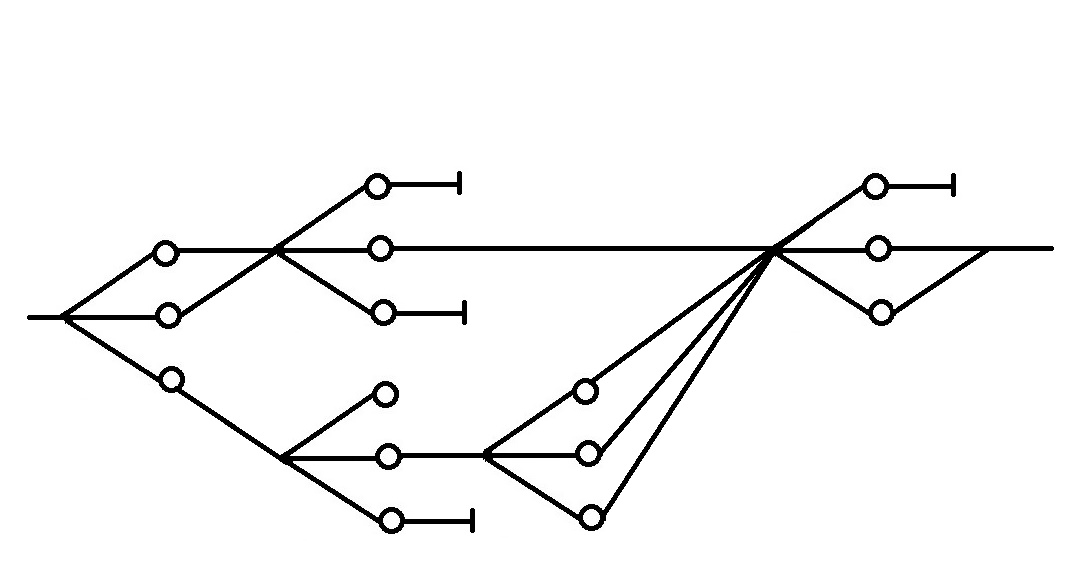
\includegraphics[scale=0.85]{Henry6.jpg}
	\begin{center}
		Decision tree for Henry VI
	\end{center}
\end{figure}

\newpage
\subsection*{} Here is an example of a choice as you would have it in game :




The true answer would be " ", and only that would earn you points for your score, but you would not know it until the end.


\section{Keeping it fun !}

\subsection*{} Keeping the experience fun was one of main goals for this application so added little animations to make our game more lively, such a as one with two swords when you launch the game, and one with a skull when you die - we have to specify we made these animations ourselves from shutterstock pictures, which were thus free from copyright.

\subsection*{}Furthermore, we tried to make the game aesthetically pleasing by using fluid animation between loadings, adding effects on buttons and having a clean, easy to understand interface.

\newpage
\section{The improvements we will make in the future}
\subsection*{}
\textit{Story Branch} is not devoid of flaws, obviously. Here is a list of things we consider to improve it :
\begin{itemize}
\item Adding an unique picture or illustration to each of the events
\item Making a save system, which you could potentially export to play on another device
\item Expanding the tree, and thus, the script
\item Making the application available on mobile phones.
\item Making our game multi-player
\item Creating a scoring chart
\item Why not a version with the French rulers ?
\item Adding links to certain terms or people
\end{itemize}

{\let\clearpage\relax \chapter{- Technical Documentation}}

\section{Les technologies utilisées}
Le but de ce projet était également de découvrir de nouvelles technologies, ainsi nous avons choisie de développer l'application
sur les technologies Web qui sont en évolution constante. La volonté de pouvoir utilisé l'application hors ligne et de pouvoir
la déployer facilement sur des machines de toutes distributions nous a amené à se tourner vers le Framework Electron, permettant
le développement d'application native à l'aide de Javascript, HTML5 et CSS3. Ainsi l'application a également l'avantage de pouvoir être portée
facilement dans une version web hébergée sur un serveur distant. Pour bénéficier de graphisme agréable et d'une expérience unifiée, nous avons
utilisé les composant web de Material-Design de Google.

\section{Structure d'une application Electron}
Le framework Electron permet d'organiser le programme comme on organiserait les sources d'une application Web classique:
\begin{itemize}
\item un dossier pour les pages HTML statiques
\item un dossier pour les styles CSS
\item un dossier pour les scripts JS
\item un fichier main.js qui est le point d'entrée du programme et qui charge les ressources nécessaires à l'exécution de l'application.
\end{itemize}

\section{Les difficultés rencontrées}
La promesse d'Electron est de pouvoir développer une application de bureau comme on développerait un site web. Mais la multiplicité des
technologies web et leurs évolutions rapide sans standard défini à l'avance pose des problèmes de compatibilités. En effet,
certain script interne des libraires d'animations de Material Design a demandé des adaptations pour fonctionner au sein de notre application.
La découverte du trio HTML/CSS/JS a également été une des difficultés à surmonter. De plus, Electron ne propose pas de moteur de template
comme Angular le fait et il a donc été nécessaire de coder la quasi totalité du site sous forme de page statique, multipliant les doublons dans le code.


{\let\clearpage\relax \chapter{- Conclusion}}
\textit{Story Branch} is a game we developed in JavaScript, HTML and CSS, whose purpose is to make you learn about the Hundred Years War by making you play as the Kings of England during that era. To do so, the goal is to stick as closely as possible to real life, which also allows to see that, sometimes, reality supersedes fiction !


{\let\clearpage\relax \chapter{- Credits:}}

We used informations from the websites listed below: \newline
History informations:
\begin{itemize}
\item \textit{https://www.shutterstock.com}
\item \textit{https://en.wikipedia.org}
\item \textit{http://www.history.com/topics/hundred-years-war}
\item \textit{http://www.bbc.co.uk/history/british/middle_ages/hundred_years_war_01.shtml}
\end{itemize}

Technologies:
\begin{itemize}
\item \textit{https://material.io/}
\item \textit{https://electron.atom.io/}
\item \textit{https://stackoverflow.com/}
\item \textit{https://www.w3schools.com/}
\end{itemize}

\end{document}
